% Created by tikzDevice version 0.12.3.1 on 2022-01-16 03:38:16
% !TEX encoding = UTF-8 Unicode
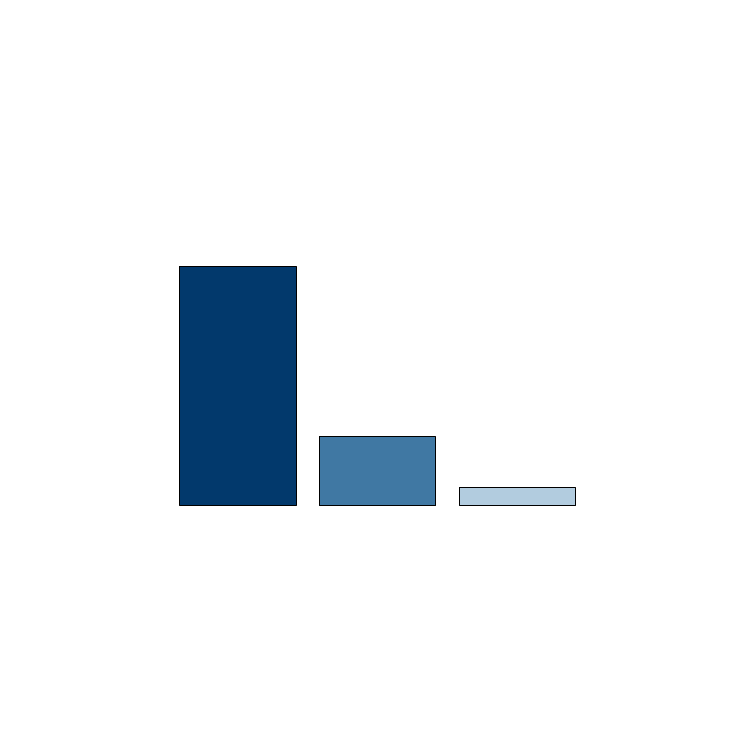
\begin{tikzpicture}[x=1pt,y=1pt]
\definecolor{fillColor}{RGB}{255,255,255}
\path[use as bounding box,fill=fillColor,fill opacity=0.00] (0,0) rectangle (252.94,252.94);
\begin{scope}
\path[clip] (  0.00,  0.00) rectangle (252.94,252.94);
\definecolor{drawColor}{RGB}{0,0,0}
\definecolor{fillColor}{RGB}{2,57,108}

\path[draw=drawColor,line width= 0.4pt,line join=round,line cap=round,fill=fillColor] ( 54.92, 80.22) rectangle ( 97.01,166.53);
\definecolor{fillColor}{RGB}{64,120,163}

\path[draw=drawColor,line width= 0.4pt,line join=round,line cap=round,fill=fillColor] (105.43, 80.22) rectangle (147.52,105.05);
\definecolor{fillColor}{RGB}{178,204,223}

\path[draw=drawColor,line width= 0.4pt,line join=round,line cap=round,fill=fillColor] (155.93, 80.22) rectangle (198.02, 86.72);
\end{scope}
\end{tikzpicture}
